\documentclass[bwprint]{gmcmthesis}
\usepackage{amsmath}
\usepackage{pdfpages}
\usepackage{graphicx}
\usepackage{subcaption}
\numberwithin{figure}{section}

\title{Computer Vision Homework 2 Report}

\author{涂宇清 522030910152}
\date{}

\begin{document}
\setlength{\parskip}{10pt}
\baselineskip=1.5\baselineskip
% \linespread{0.1}
\maketitle

\section{Programming Assignment}
\begin{enumerate}
    \item In \verb|init_world_points()|, we use \verb|cv2.findChessboardCorners()| to find the corners of the chessboard. And we use \verb|cv2.cornerSubPix()| to refine the corner positions. We store the 3D world points and 2D image points in \verb|world_points| and \verb|image_points| respectively.
    \item As we have learnt in class, we can get $H$ of each picture by eigenvalue decomposition. And we can also get $B$ from $H$ by eigenvalue decomposition. Then, using Cholesky factorization, we can get $K$, which is the intrinsic matrix.
    \item Then, we can use $P$, the camera matrix, to get reprojection error of each image.
\end{enumerate}

\begin{figure}[htpb]
    \centering
    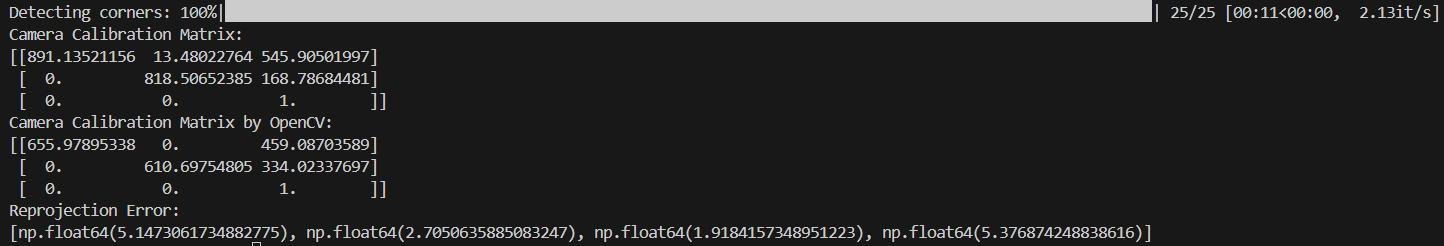
\includegraphics[width=\textwidth]{pictures/result.png}
    \caption{Results of camera calibration.}
    \label{fig:results}
\end{figure}

The results are shown in Figure \ref{fig:results}.


\section{Written Assignment}
\subsection{Problem 1}
\begin{enumerate}[label=\alph*.]
    \item 
    \begin{align}
        E(A, T) &= \sum_{i=1}^{N}||Y_i - AX_i - T||_2^2 \notag \\
                &= \sum_{i=1}^{N}(Y_i - AX_i - T)^T(Y_i - AX_i - T) \notag
    \end{align}
    To minimize $E(A, T)$, we need to take the derivative of $E(A, T)$ with respect to $A$ and $T$ and set them to zero.
    \begin{align}
        \frac{\partial E(A, T)}{\partial A} &= \sum_{i=1}^{N}2(AX_i + T - Y_i)X_i^T = O \notag \\
        \frac{\partial E(A, T)}{\partial T} &= \sum_{i=1}^{N}2(AX_i + T - Y_i) = O \notag
    \end{align}
    It is given by the second equation that $T = \frac{1}{N}\sum_{i=1}^{N}(Y_i-AX_i) = \hat{Y} - A\hat{X}$
    Then we can substitute $T$ with $\hat{Y} - A\hat{X}$ in the first equation and get 
    \begin{align}
        \sum_{i=1}^{N}(AX_i + \hat{Y} - A\hat{X} - Y_i)X_i^T &= O \notag \\
        A\sum_{i=1}^{N}(X_i - \hat{X})X_i^T &= \sum_{i=1}^{N}(Y_i - \hat{Y})X_i^T \notag
    \end{align}
    And we know that
    \begin{align}
        \sum_{i=1}^{N}(X_i - \hat{X})(X_i - \hat{X})^T &= \sum_{i=1}^{N}(X_i - \hat{X})X_i^T - \sum_{i=1}^{N}(X_i - \hat{X})\hat{X}^T \notag \\
        &= \sum_{i=1}^{N}(X_i - \hat{X})X_i^T - \left(\sum_{i=1}^{N}X_i\hat{X}^T - N\hat{X}\hat{X}^T\right) \notag \\
        = \sum_{i=1}^{N}(X_i - \hat{X})X_i^T \notag
    \end{align}
    and
    \begin{align}
        \sum_{i=1}^{N}(Y_i - \hat{Y})(X_i - \hat{X})^T = \sum_{i=1}^{N}(Y_i - \hat{Y})X_i^T \notag
    \end{align}
    So we can get
    \begin{align}
        A\sum_{i=1}^{N}(X_i - \hat{X})X_i^T &= \sum_{i=1}^{N}(Y_i - \hat{Y})X_i^T \notag \\
        A\sum_{i=1}^{N}(X_i - \hat{X})(X_i - \hat{X})^T &= \sum_{i=1}^{N}(Y_i - \hat{Y})(X_i - \hat{X})^T \notag \\
        A(XX^T) &= YX^T \notag \\
        A &= (YX^T)(XX^T)^{-1} \notag
    \end{align}
    To sum up, $\min(E(A, T))$ is given by $T^* = \hat{Y} - A^*\hat{X}$, $A^* = (YX^T)(XX^T)^{-1}$.
    \item For every correspondence $(x_i, y_i)$, we have
    \begin{align}
        y_i &= Ax_i + T \notag \\
        \begin{bmatrix}
            y_1 \\
            y_2 \\
            y_3
        \end{bmatrix} &= \begin{bmatrix}
                A_{11} & A_{12} & X_{13} \\
                A_{21} & A_{22} & X_{23} \\
                A_{31} & A_{32} & X_{33}
            \end{bmatrix}
            \begin{bmatrix}
                x_1 \\
                x_2 \\
                x_3
            \end{bmatrix} +
            \begin{bmatrix}
                T_1 \\
                T_2 \\
                T_3
            \end{bmatrix} \notag
    \end{align}
    three equations totally. And $A$ and $T$ have 12 unknowns. So we need at least 4 correspondences to estimate the transformation.
\end{enumerate}

\end{document} 
